\SetKwProg{Proc}{procedure}{}{}
\SetKwFunction{Search}{SEARCH}
\SetKwFunction{SampleParticle}{SAMPLE-PARTICLE}
\SetKwFunction{Simulate}{SIMULATE}
\SetKwFunction{Timeout}{TIMEOUT}
\SetKwFunction{Maxstep}{MAX-STEP}
\SetKwFunction{SearchBest}{SEARCH-BEST}
\SetKwFunction{UCB}{UCB}
\SetKwFunction{Rollout}{ROLLOUT}
\SetKwFunction{UpdateBelief}{UPDATE-BELIEF}
\SetKwFunction{ComputeConfidence}{CONF}
\SetKwFunction{SelectBestHypothesis}{SELECT-FACT}
\SetKwFunction{QuerySource}{QUERY}
\SetKwFunction{FilterBelief}{FILTER}

\section{Belief-Guided State Verification}~\label{method:system_architecture}
The proposed method uses a belief over symbolic successor states to coordinate two feedback decisions: when additional information is necessary and what state information should be requested. After each robot action and observation, the method constructs a weighted set of reachable symbolic worlds. Belief confidence determines whether execution can continue without external information. If confidence is insufficient, the method selects a predicate fact according to its expected reduction in belief entropy, queries an external source, and removes worlds inconsistent with the answer. The robot then commits to the most probable remaining state and retains responsibility for subsequent action selection.

\subsection{Method Overview}~\label{method:overview}
Fig.~\ref{fig:pm} shows the execution loop. Let $s_t^{K}$ denote the symbolic state currently committed for planning. The POMCP planner selects an applicable robot action $a_t$, which is executed to obtain observation $o_{t+1}$. The transition and observation models induce a posterior belief $\mathcal{B}_{t+1}$ over reachable successor states. The method then applies the following sequence:
\[
s_t^{K}
\xrightarrow[\text{execute}]{a_t}
\mathcal{B}_{t+1}
\xrightarrow[\text{when}]{\mathrm{Conf}}
\xrightarrow[\text{what}]{\text{expected entropy}}
\widehat{s}_{t+1}^{K}.
\]
The middle two operations are the feedback policy studied in this paper. If no query is triggered, or after the query loop terminates, the maximum a posteriori world becomes the committed state $\widehat{s}_{t+1}^{K}$ for the next planning step.

\begin{figure}[t]
\captionsetup{skip=0pt}
\centering
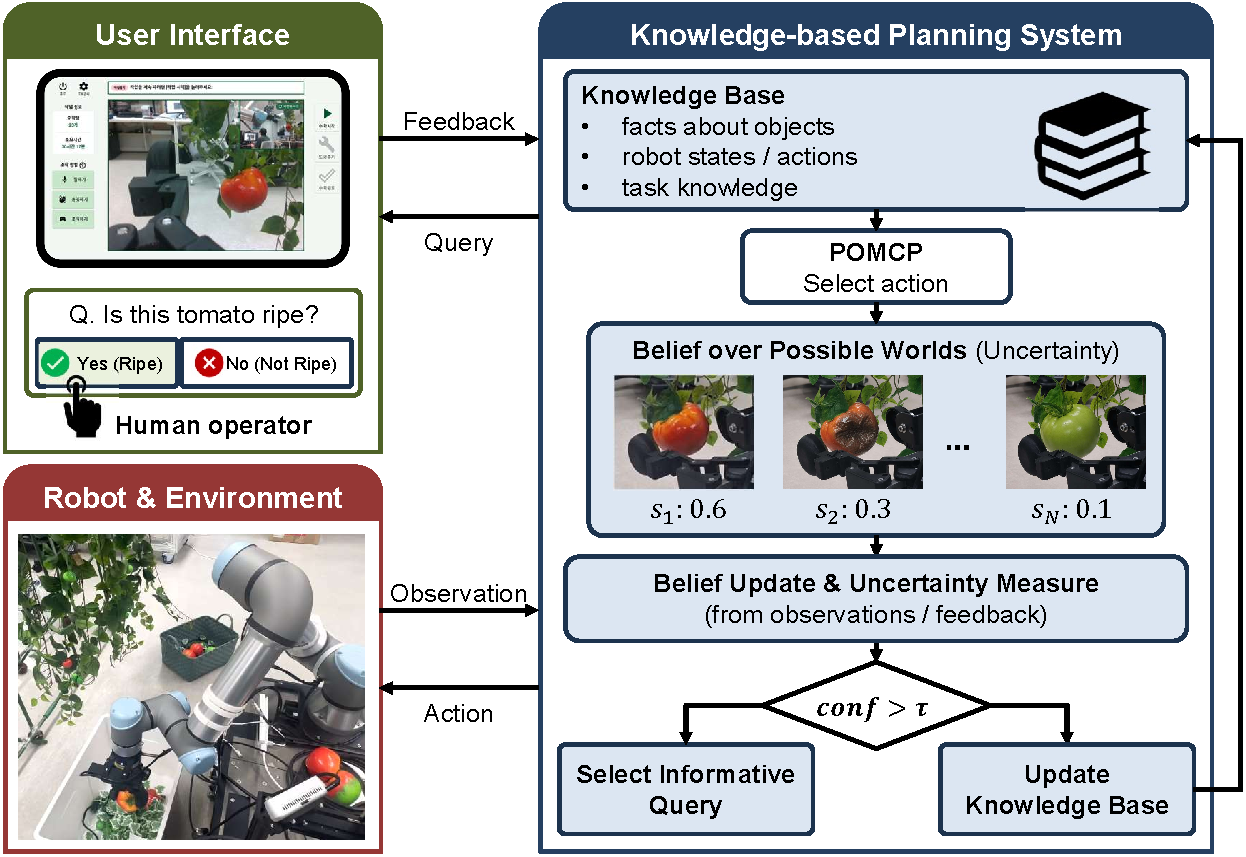
\includegraphics[width=0.98\linewidth]{figures/fig_overview.pdf}
\caption{Belief-guided state-verification loop. A robot action and observation produce a weighted frontier of reachable symbolic worlds. Belief confidence determines when to request external information, and expected posterior entropy determines which predicate fact to verify. The answer refines the belief before the robot selects its subsequent action.}
\label{fig:pm}
\end{figure}

\subsection{Reachable Symbolic Belief}~\label{method:belief_rep}
The state representation combines symbolic facts with numeric fluents. Facts encode task conditions that affect action applicability, such as $\texttt{ripe}(\text{tomato}_1)$ or an object's waste category. Numeric fluents encode quantities used by robot skills, such as object poses and distances. The feedback policy reasons over uncertainty in symbolic facts; numeric values are updated from sensing without expanding the symbolic hypothesis set.

Rather than maintaining a global belief over every logically possible world, the method constructs a local \emph{frontier} after each executed action. Given committed state $s_t^{K}$ and action $a_t$, the transition model returns the symbolic successors with nonzero probability:
\begin{equation}
\mathcal{F}_{t+1}
=
\mathrm{Frontier}(s_t^{K},a_t)
=
\{s_{t+1}^{1},\ldots,s_{t+1}^{j}\}.
\label{eq:frontier}
\end{equation}
Deterministic add and delete effects are applied directly, while uncertain outcomes instantiate mutually exclusive successor hypotheses defined by the domain model. Duplicate successors are merged. If the number of outcomes exceeds the particle budget, successors are sampled without replacement according to their transition probabilities. This construction restricts feedback decisions to states reachable from the current planning context.

After receiving observation $o_{t+1}$, each frontier state is weighted using both its transition probability and its action-conditioned observation likelihood:
\begin{equation}
\begin{aligned}
\bar{w}_{k}
&=T(s_{t+1}^{k}\mid s_t^{K},a_t)\,
O(o_{t+1}\mid s_{t+1}^{k},a_t),\\
w_k&=\frac{\bar{w}_k}{\sum_{\ell=1}^{j}\bar{w}_{\ell}}.
\end{aligned}
\label{eq:belief_update}
\end{equation}
If every unnormalized weight is zero, the implementation falls back to a uniform distribution over the represented frontier. The resulting belief is
\begin{equation}
\mathcal{B}_{t+1}
=
\{(s_{t+1}^{k},w_k)\}_{k=1}^{j},
\qquad
\sum_{k=1}^{j}w_k=1.
\label{eq:symbolic_belief}
\end{equation}
This explicit weighted frontier is used for confidence estimation and query selection. POMCP separately maintains sampled states in its search tree for action-value estimation; both components use the same symbolic transition and observation models.

\subsection{When to Query: Belief Confidence}~\label{method:uncertainty}
The timing policy asks whether the posterior belief is sufficiently concentrated to continue execution. Its entropy is
\[
\mathcal{H}(\mathcal{B}_{t+1})
=
-\sum_{k=1}^{j}w_k\log_2 w_k.
\]
Because the maximum entropy depends on the number of represented worlds, we normalize by $\log_2 j$ and define
\begin{equation}
\mathrm{Conf}(\mathcal{B}_{t+1})
=
1-\frac{\mathcal{H}(\mathcal{B}_{t+1})}{\log_2 j}.
\label{eq:compute_confidence}
\end{equation}
For $j=1$, we define $\mathrm{Conf}(\mathcal{B}_{t+1})=1$. The score approaches zero when the represented worlds have similar weights and approaches one when the posterior concentrates on one world.

Given threshold $\tau\in[0,1]$, the robot initiates state verification when
\begin{equation}
\mathrm{Conf}(\mathcal{B}_{t+1})<\tau.
\label{eq:when_query}
\end{equation}
Thus, $\tau$ controls the empirical trade-off between acting with unresolved state ambiguity and acquiring additional information. The policy is deliberately based on uncertainty in the current symbolic state, rather than confidence in a generated action label. Its effect on task success is evaluated by varying $\tau$ and by comparing uncertainty-based timing with dense, absent, and random feedback schedules.

\subsection{What to Query: Expected Entropy Reduction}~\label{method:query_selection}
Once a query is triggered, the method selects a symbolic fact that distinguishes the remaining worlds. Let $\mathcal{C}(\mathcal{B})$ contain every fact that holds in at least one, but not all, frontier states:
\[
\mathcal{C}(\mathcal{B})
=
\left\{
c\in\mathcal{F}
\;\middle|\;
0<\sum_{k:c\in s^k}1<j
\right\}.
\]
For candidate $c$, the belief is partitioned according to its truth value:
\[
\begin{aligned}
\mathcal{B}_{c}^{+}&=\{(s^k,w_k)\mid c\in s^k\},\\
\mathcal{B}_{c}^{-}&=\{(s^k,w_k)\mid c\notin s^k\}.
\end{aligned}
\]
Let $P(c)=\sum_{k:c\in s^k}w_k$ and $P(\neg c)=1-P(c)$. Entropy within each subset is computed after conditionally normalizing its weights. The expected posterior entropy of asking about $c$ is
\[
\mathbb{E}[\mathcal{H}\mid c]
=
P(c)\mathcal{H}(\mathcal{B}_{c}^{+})
+
P(\neg c)\mathcal{H}(\mathcal{B}_{c}^{-}).
\]
The selected query is
\begin{equation}
c^*
=
\arg\min_{c\in\mathcal{C}(\mathcal{B})}
\left[
P(c)\mathcal{H}(\mathcal{B}_{c}^{+})
+
P(\neg c)\mathcal{H}(\mathcal{B}_{c}^{-})
\right].
\label{eq:select_hypo}
\end{equation}
Equivalently, Eq.~\ref{eq:select_hypo} maximizes one-step information gain because the current belief entropy is fixed across candidates. The criterion is recomputed after every answer, so successive questions adapt to the remaining worlds. The content-selection experiments test whether this targeted choice reduces the number of queries relative to selecting a differentiating fact at random.

\subsection{Feedback Update and Online Execution}~\label{method:planning}
The selected predicate is converted into a binary state-verification query. For example, $c^*=\texttt{ripe}(\text{tomato}_1)$ produces the question \emph{Is tomato 1 ripe?} The answer $y\in\{\texttt{true},\texttt{false}\}$ filters the belief:
\begin{equation}
\mathcal{B}
\leftarrow
\begin{cases}
\{(s^k,w_k)\mid c^*\in s^k\}, & y=\texttt{true},\\
\{(s^k,w_k)\mid c^*\notin s^k\}, & y=\texttt{false}.
\end{cases}
\label{eq:filter}
\end{equation}
The retained weights are renormalized, confidence is recomputed, and another fact is selected if confidence remains below $\tau$. The loop stops when the threshold is met or no differentiating fact remains. The robot then commits the maximum a posteriori state
\[
s_{t+1}^{K}
=
\arg\max_{s^k\in\mathcal{B}_{t+1}}w_k
\]
for subsequent planning. We call this a committed planning state rather than a certain state: it is the hypothesis used by the next planning step after the available sensing and feedback have been incorporated.

Algorithm~\ref{alg:online_planning} summarizes the complete interaction between planning and state verification. The feedback update treats an answer as hard evidence. Consequently, an incorrect answer can remove the true world if it is present in the frontier; the oracle evaluation isolates the query policy under correct feedback, while the VLM and user evaluations examine its behavior with realistic feedback sources.

\begin{algorithm}[t]
\caption{Belief-Guided State Verification and Planning}
\label{alg:online_planning}
\textbf{Input}: initial state $s_0^{K}$, confidence threshold $\tau$, step limit $T_{\max}$\\
\textbf{Output}: executed action sequence $\pi$
\BlankLine
$\mathcal{B}\gets\{(s_0^{K},1)\}$; $t\gets0$; $\pi\gets()$\\
\While{$t<T_{\max}$}{
    $a_t\gets$\Search{$\mathcal{B}$}\label{alg1_planning:search}\\
    \If{$a_t=\emptyset$}{
        \textbf{break}\tcp*{dead end}
    }
    execute $a_t$ and receive $o_{t+1}$\\
    $\pi\gets\pi\mathbin{\|}a_t$\\
    $\mathcal{B}\gets$\UpdateBelief{$s_t^{K},a_t,o_{t+1}$}\label{alg1_planning:belief_update}\\
    $q\gets\mathrm{Conf}(\mathcal{B})$\label{alg1_planning:compute_conf}\\
    \While{$q<\tau$}{
        $c^*\gets$\SelectBestHypothesis{$\mathcal{B}$}\label{alg1_planning:select_hypo}\\
        \If{$c^*=\emptyset$}{
            \textbf{break}\tcp*{no differentiating fact}
        }
        $y\gets$\QuerySource{$c^*$}\\
        $\mathcal{B}\gets$\FilterBelief{$\mathcal{B},c^*,y$}\label{alg1_planning:filter}\\
        $q\gets\mathrm{Conf}(\mathcal{B})$\\
    }
    $s_{t+1}^{K}\gets\arg\max_{s^k\in\mathcal{B}}w_k$\\
    $t\gets t+1$\\
}
\KwRet $\pi$
\end{algorithm}

\begin{figure*}[t!]
\captionsetup{skip=0pt}
\centering
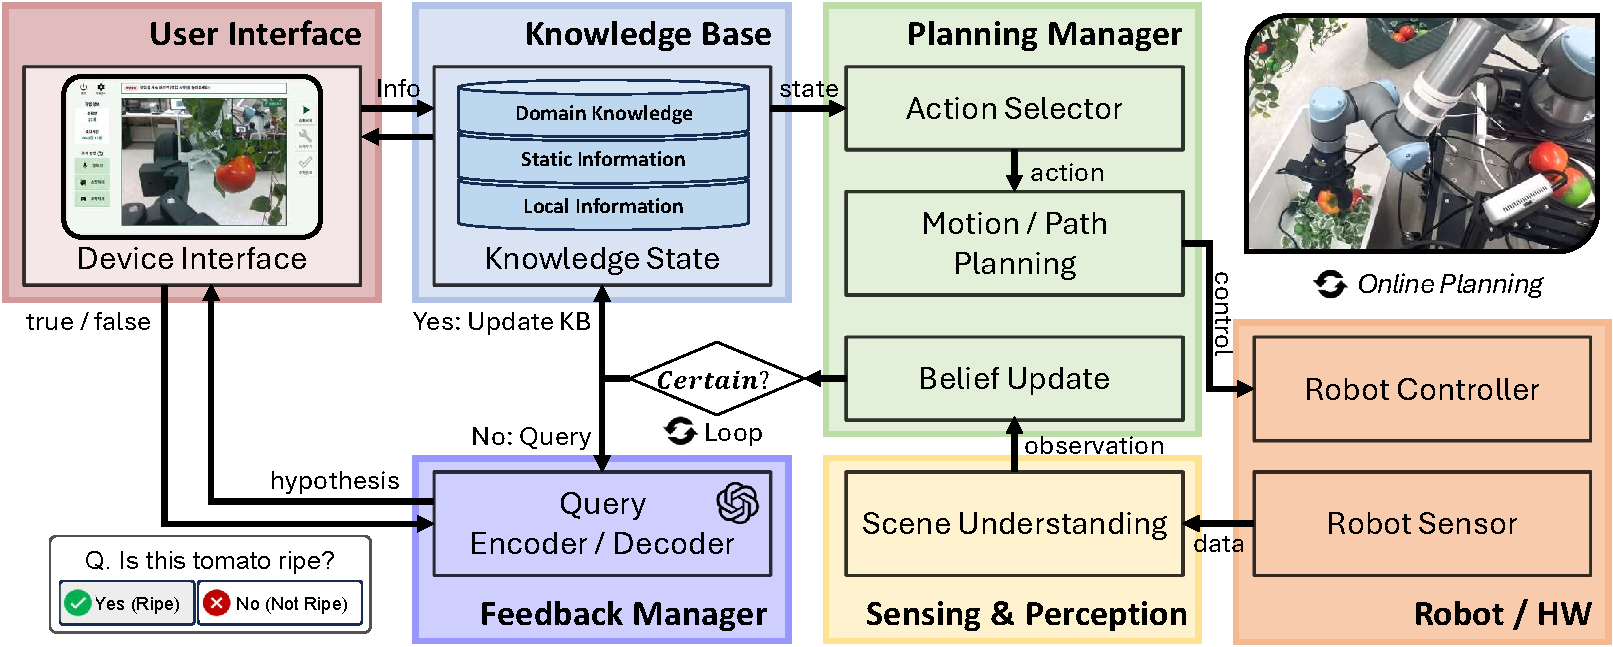
\includegraphics[width=0.95\linewidth]{figures/fig_dataflow.pdf}
\caption{System realization of the belief-guided state-verification method. The KB shares task facts and action models across planning, sensing, and feedback. The PM retains action selection, while the FM and UI acquire external evidence about a selected symbolic fact.}
\label{fig:data_flow}
\end{figure*}

\subsection{Integration with Symbolic POMCP}~\label{method:PM}
We use POMCP~\cite{silver2010monte} to select robot actions from the current belief. The search retains the standard simulation and value-update structure, but restricts both tree expansion and rollout to actions whose symbolic preconditions hold in the sampled state. Given state $s$, the planner therefore explores
\[
\mathcal{A}(s)=\{a\in\mathcal{A}\mid \mathrm{pre}(a)\subseteq s\}
\]
rather than the full action set. The generative model samples $(s',o,r)$ from the same domain transition and observation models used to construct the explicit frontier. This avoids evaluating symbolically infeasible actions while preserving stochastic search over reachable outcomes.

After an action, observation, and any external feedback have been incorporated, the search tree is pruned using the executed action and the committed successor state. The subsequent search therefore begins from the state estimate produced by the full sensing-and-verification loop. Detailed search, simulation, and rollout pseudocode is provided in Appendix~\ref{appx:algorithms}; these routines support action selection but are not the feedback policy studied in the main experiments.

\subsection{System Realization}~\label{method:modules}
The method is realized through the modules shown in Fig.~\ref{fig:data_flow}. The Knowledge Base (KB) provides the shared symbolic state and action model. The Planning Manager (PM) performs POMCP search, constructs and updates the reachable frontier, and invokes the feedback policy. Sensing and Perception (SP) supplies observations and numeric state estimates. The Feedback Manager (FM) formats the selected predicate and incorporates the response, while the User Interface (UI) presents state-verification questions during human interaction.

\subsubsection{Knowledge Representation and Perception}~\label{method:KB}
The KB partitions information into domain knowledge $\mathcal{I}^{D}$, static structured information $\mathcal{I}^{S}$, and local information $\mathcal{I}^{L}$ obtained during execution:
\[
\mathcal{KB}=\mathcal{I}^{D}\sqcup\mathcal{I}^{S}\sqcup\mathcal{I}^{L}.
\]
Domain knowledge contains action schemas and task rules. Static information includes invariant facts and fixed map or robot parameters. Local information contains perceptual facts and numeric fluents that are updated during execution. SP maps raw sensor input to these task-level observations. For example, RGB-D sensing can update object pose and ripeness estimates, while the symbolic observation likelihood determines how those observations weight the frontier states.

\subsubsection{Robot Action Execution}~\label{method:action_execution}
Each symbolic action is associated with an executable robot skill. Actions such as $\texttt{navigate}(\text{robot},l_1,l_2)$ and $\texttt{pick}(\text{robot},\text{tomato}_1)$ specify task-level intentions, while an off-the-shelf motion planner such as MoveIt~\cite{chitta2012moveit} uses numeric fluents from the KB to generate low-level motion. This separation allows the feedback policy to operate on task-level facts without depending on a particular motion-planning implementation.

\subsubsection{Feedback Interface}~\label{method:FM}
The FM maps the selected predicate to a predefined question template and converts the response to a Boolean value. During human interaction, the tablet UI displays the camera view, highlights the referenced object with a bounding box, and presents simple response options, as shown in Fig.~\ref{fig:FM_UI}. The interface exposes the state fact being verified but does not ask the user to choose the robot's next action.

\begin{figure}[H]
\captionsetup{skip=0pt}
\centering
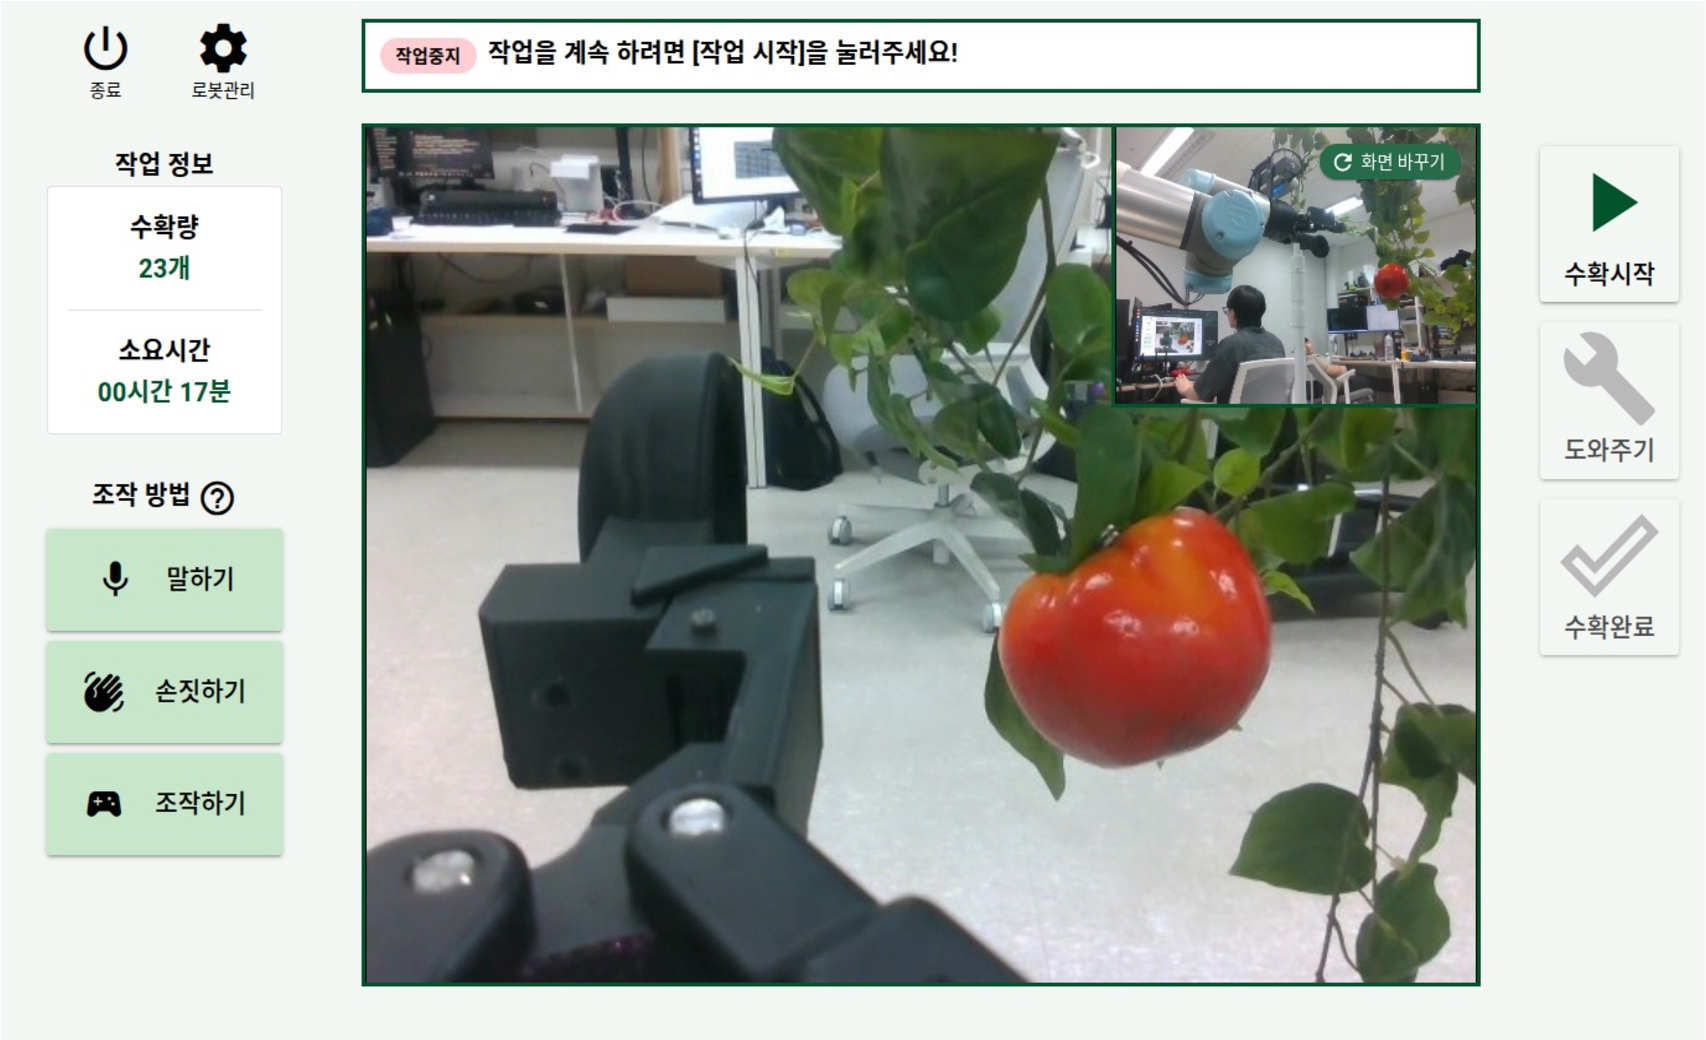
\includegraphics[width=\linewidth]{figures/fig_interface.pdf}
\caption{State-verification interface. The queried object and response options provide evidence for filtering the symbolic belief.}
\label{fig:FM_UI}
\end{figure}
